\chapter{Diseño de la solución}\label{chap:Design}
En este capítulo se describirá el modo en el que la API para la interconexión entre el simulador y el juego será construida y cómo este ha de ser llevado a cabo para cumplir con los propósitos que se han ido repitiendo a lo largo del texto.

\section{La API: GNS3sharp}\label{sec:dis_api}
Para llevar a cabo la interacción entre el videojuego y el simulador de redes es necesario desarrollar previamente alguna herramienta que lo posibilite. Con este fin, se ha construido una librería propia que ofrece configurar y obtener información del simulador desde fuera de él.

\begin{figure}[H]
  \centering
  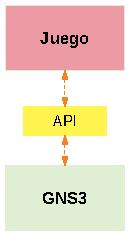
\includegraphics[scale=1.4]{imagenes/capa_api}
  \caption{La API en el proyecto}
  \label{fig:capa_api}
\end{figure}

Esta librería será usada mediante una API, que en nuestro proyecto se encuentra, de forma lógica, entre el juego y GNS3 tal y como se esquematiza en la figura \ref{fig:capa_api}. Todos sus detalles serán explicados en las próximas páginas.

\subsection{Introducción}\label{subsec:sectionapi}
Según Wikipedia, una \textbf{API} ``es un conjunto de subrutinas, funciones y procedimientos (o métodos, en la programación orientada a objetos) que ofrece cierta biblioteca para ser utilizado por otro software como una capa de abstracción''\cite{wiki:api}. Comprende una serie de funciones que facilitan en mayor o menor medida trabajar sobre un cierto elemento. Como ejemplo de API famosa tenemos la de Google Maps, que contiene un compendio de métodos para JavaScript que permiten interactuar directamente con la plataforma de Google y crear nuestros programas jugando con ella\cite{googlemaps}. En resumen, una API no es más que un conjunto de funciones definidas para acceder a un servicio determinado.

En la programación de sistemas complejos se suele aplicar un diseño basado en \textbf{capas de abstracción}. Partiendo de conceptos concretos se desarrolla una capa de abstracción haciendo uso de ellos que permite elevar el trato de elementos concretos un nivel por encima\cite{abstraction}. De esta forma ganamos en agilidad de escritura y sencillez en el diseño sin perder flexibilidad de desarrollo.

Como se ha citado previamente, GNS3 implementa una \textbf{API REST} (\textit{REpresentational State Transfer}). Esto es, mediante una serie de métodos (los conocidos GET, POST...) asociados a una URI (\textit{Uniform Resource Identifier} o identficador de recurso uniforme \cite{uri}) concreta podemos interactuar \textbf{vía web} con una aplicación. La diferencia fundamental con otra clase de servicios web es que REST está orientado a recursos y no a métodos. Esto permite a la web utilizar comunicaciones sin estado, facilitando de este modo su escalabilidad\cite{REST}.

Aunque de gran utilidad (ya que permite tomar información de los proyectos de GNS3 y controlar algunos de sus parámetros), hace falta algo más para poder propiciar la interacción entre el simulador de redes y el videojuego; la API trabaja a un nivel mucho más bajo del que requerimos para desarrollar los juegos. Surge la necesidad entonces de crear nuestra propia API que haga uso de la API REST de GNS3 y que defina las funciones necesarias, a un nivel más abstracto y con más facilidades, que haga de intermediaria entre GNS3 y Unity.

\subsection{Elección del lenguaje para la librería}
En pleno 2018, la cantidad de lenguajes de programación existentes roza el absurdo. Desde el tradicional C, pasando por el multifuncional Java, el sencillo Python o incluso los llamados lenguajes esotéricos como LOLCODE\cite{esotericlang}. Nosotros elegiremos uno sobre el que trabajar de entre todos ellos. Esta decisión está condicionada, como es natural, por el motor de videojuegos a utilizar.

Ya que nuestra intención es que el motor sea capaz de establecer interacción con el simulador, es necesario que la API a desarrollar esté escrita en un lenguaje con el que el propio motor sea capaz de trabajar. \textbf{C\#} parecía la opción más sensata. ¿Por qué? Las razones se exponen a continuación:

\begin{itemize}
\item\textbf{Porque es el lenguaje más usado en Unity}. Unity admite varios lenguajes de programación con los que desarrollar los scripts asociados a los juegos. C++, usado en otros muchísimos otros motores de videojuegos como Unreal Engine, es uno de ellos. Aunque se trate de un lenguaje increíblemente potente y eficiente, su complejidad de uso es mucho mayor, ya que se encuentra a más bajo nivel. JavaScript es otro de ellos, pero no es tan recomendable como C\#, pues entre otras razones, a diferencia de JS, C\# es fuertemente tipado\cite{unityinaction}. En general, C\# es el lenguaje usado por defecto en Unity y el recomendado por todos, documentación incluida.
\item\textbf{Porque es utilizado por varios motores}. Unity está en el podio de entre los motores de videojuegos más usados en el mundo. Como tal se convierte en un referente. El resto de motores miran hacia él y, si quieren atraer a nuevos programadores, tendrán que hacer de su incursión en el nuevo motor algo sencillo. Este es el caso de Godot Engine, que unos meses atrás decidió incluir tal lenguaje entre los soportados\cite{godotcs}. Esto quiere decir que la API no solo podrá ser usada en juegos creados en Unity, si no que su terreno de juego se verá ampliado. CryEngine es otro de los motores que permiten el uso de C\# como lenguaje de scripting.
\item\textbf{Porque, ante todo, se trata de un lenguaje versátil y robusto}. C\#, similar en cuanto a sintaxis a Java, nació como respuesta a este de la mano de Microsoft. Se trata de un lenguaje de propósito general, aunque es usado primordialmente para la construcción de aplicaciones para infraestructuras Windows. Es uno de los lenguajes que componen la plataforma .NET de Microsoft. Tal es su importancia que a día de hoy se posiciona como el cuarto lenguaje de programación más usado a nivel mundial\cite{csisfamous}. Alguna de las características que lo hacen especialmente atractivo:
\begin{itemize}
\item Es un \textbf{lenguaje de programación orientado a objetos}, con lo que posee todas las características propias de estos (encapsulado, herencia y poliformismo). Sin embargo, no admite multiherencia. Su componente fundamental es una unidad de encapsulamiento de datos y
funciones llamada \texttt{type} o ``tipo''. C\# tiene un sistema de tipos unificado, donde todos los tipos en última instancia comparten un tipo de base común.
\item Aunque es principalmente un lenguaje orientado a objetos, también \textbf{toma prestado del paradigma de programación funcional}. Las funciones pueden ser tratadas como valores mediante el uso de delegados, permite el uso de expresiones lambda, acercándose a los patrones declarativos del paradigma funcional...
\item Admite \textbf{tipado estático}, lo cual se traduce en que el lenguaje obliga a que haya coherencia entre los tipos durante el tiempo de compilado. El tipado estático elimina un gran número de errores antes de que se ejecute un programa. Desplaza la carga del momento de la ejecución hacia el compilador para verificar que todos los tipos en un programa encajan correctamente. Esto hace que las aplicaciones grandes sean mucho más fáciles de administrar, más predecibles y más robustas. Además, la escritura estática permite que herramientas como IntelliSense en Visual Studio ayuden a desarrollar, pues conoce el tipo de una variable determinada y, por lo tanto, qué métodos puede utilizar está habilitada a usar. C\# incluye además el tipo \texttt{dynamic} que permite sortear el tipado estático y dejar que el tipo de variable se averigüe durante el momento de la ejecución\cite{csnutshell}.
\end{itemize}
Particularmente, en este trabajo adoptaremos C\#7, lanzado a la vez que Visual Studio 2017. Entre sus características más interesantes se incluye la aparición de tuplas, especialmente útil cuando queremos devolver más de una variable como resultado de una función.
\end{itemize}
Aclarada las razones, pasamos a analizar el uso que le daremos a este lenguaje.

\subsection{Diseño de la API}
Antes de desarrollar la API es necesario reflexionar sobre los distintos aspectos que la compondrán (estructura, servicios, funciones...). Se ha decidido darle por nombre \textbf{GNS3sharp}, por la fusión entre las dos tecnologías que la conforman. Para dar soluciones, tenemos que plantearnos antes las preguntas adecuadas:
\subsubsection[Interacción con GNS3]{Interacción con GNS3 (¿Cómo debe interactuar con el simulador?)}
Como ya se dijo con anterioridad, GNS3 crea un servidor en el equipo desde el que se ejecuta. Este servidor acepta peticiones REST, creando así una suerte de interacción con el programa sin necesidad de poner las manos en él de forma directa. Se abre de esta forma al mundo del scripting y así a nosotros para crear un conjunto de métodos que faciliten su acceso y gestión. Todo esto volverá a ser ilustrado en la subsección \ref{subsec:interac_emul} con mayor detalle.

Tratándose de una API REST, lo único que nos es necesario para la conexión es un \textbf{cliente web}. El framework de .NET ya cuenta con una clase dedicada a ello denominada \texttt{System.Net.WebClient}\cite{webclient}, que contiene métodos más que suficientes para nuestro uso. Será pues sobre esto sobre lo que se base primordialmente la relación entre nuestra librería y el simulador de redes como tal. A continuación veremos que habremos de emplear alguna tecnología más.

\subsubsection[Acceso a la API]{Acceso a la API (¿Cómo queremos que interactúe con el exterior?)}\label{subsec:accesoapi}
Es importante tener esto claro, pues el uso de la librería y de sus métodos por parte de una aplicación externa debe optimizar la productividad y agilizar el desarrollo lo máximo posible. Aquel que vaya a hacer uso de ellas debe tener un esquema claro del modo en que puede gestionar la interacción, siendo pues cercana al usuario (más bien desarrollador) último.

GNS3 funciona a través de proyectos. En un proyecto se pueden incluir tantos nodos como se desee para, a posteriori, ser interconectados. Las posibilidades son muy amplias y dejan poder absoluto al usuario. La singularidad del proyecto apenas pasa por permitir arrancar o apagar todos los nodos contenidos en él a la vez.

Siendo así, se ha optado por concentrar lo crucial de la interacción entre el simulador y el desarrollador en \textbf{una sola clase-objeto}. Esta clase, que se explicará con detalle más adelante, permitirá hacer de puente entre el proyecto y los distintos elementos que lo componen y aquel que haga uso de ella.

\subsubsection[Funcionalidad]{Funcionalidad (¿Qué queremos que haga?)}
Todo lo explicado hasta ahora es correcto: definimos una forma con la que el código pueda acceder al simulador y reflexionamos en la manera en la que el desarrollador que la use pueda sacarle partido. Sin embargo, ¿qué significa entonces \textit{sacarle partido}?

Para responder no hay más que irse al propio GNS3 y ver todas las opciones que nos ofrece: desplegar nodos, enlazarlos entre sí, cortar esos enlaces, arrancar todos los nodos juntos, parar algunos de ellos a voluntad... 

Y por supuesto y aún más importante, \textbf{gestionar los aparatos desplegados desde dentro}. Es aquí donde está su verdadero potencial. Manejar un switch conectado a varios PCs, modificar sus VLANs dinámicamente; un router conectado a varias redes distintas, desactivando y activando algunas de ellas en función de un booleano con el que estemos trabajando... Y todo esto sin necesidad de acceder a GNS3 directamente; todo mediante scripting. ¡Se abre un mundo de posibilidades!

\subsection{Diseño de clases}
Nuestra API hará uso de todas las características propias de los lenguajes orientados a objetos ya expuestas. A nivel de estructura, la que nos interesa citar ahora es la \textbf{herencia}.

La herencia es un mecanismo por el que una clase hija (llamémosla \texttt{B}) va a heredar los métodos y las propiedades de una clase padre (llamémosla \texttt{A}). La cantidad de elementos heredados entre padre e hijo puede ser determinado mediante el uso de modificadores de acceso. Como dato adicional, este lenguaje no admite herencia de constructores, así que nuestra clase \texttt{B} tendrá que definir su propio constructor (o bien explicitar su herencia respecto al de \texttt{A}).

Aclarado el concepto, mostramos la estructura básica sobre la que nuestra librería será construida:

\begin{figure}[H]
  \centering
  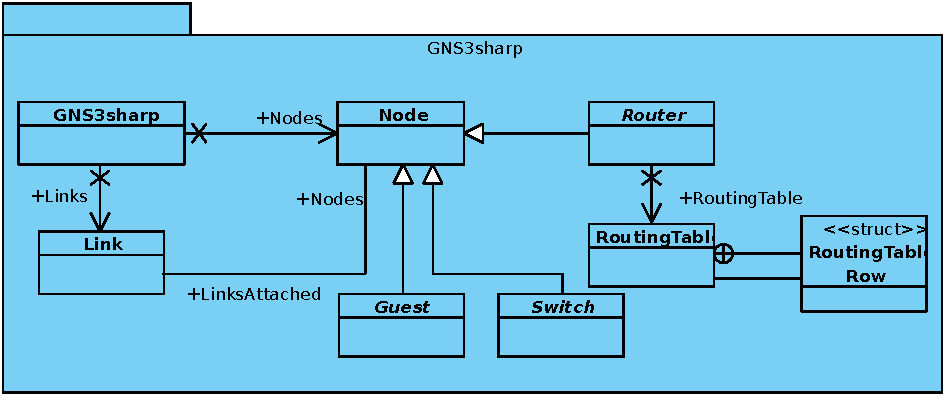
\includegraphics[scale=0.75]{imagenes/diagrama_api1}
  \caption{Esquema de diagrama UML de la API}
  \label{fig:diagrama_api1}
\end{figure}

El diagrama UML de la figura \ref{fig:diagrama_api1} dibuja cuáles son las clases que componen la librería y da pistas acerca de la relación entre ellas. Así, es claro que las tales \texttt{Switch}, \texttt{Node} y \texttt{Router} heredan de de \NODE~y que a su vez esta es usada por \GNSCS~por alguna propiedad llamada \texttt{Nodes} (que hasta la subsección \ref{subsec:gnscsclass} no se analizará).

A continuación pasamos a desarrollar cada una de las clases conceptualmente:

\subsubsection[''La clase principal'']{GNS3sharp, la clase principal}
Tal y como expusimos en la sección~\ref{subsec:accesoapi}, crearemos una clase principal que gestionará toda la interacción con el simulador de redes. Hemos llamado a esta clase del mismo modo que a la API, \GNSCS. Recalcamos entonces: los objetos que se encarguen de gestionar los proyectos serán del tipo \GNSCS.

¿Y en qué consistirá esta gestión concretamente? Básicamente, la clase debe encargarse de:
\begin{enumerate}
\item Establecer la conexión con el servidor de GNS3 y recopilar toda la información acerca del proyecto que se pretende controlar.
\item Convertir toda es información en objetos útiles que puedan ser utilizados.
\item Crear una gestión eficiente de esos recursos de manera que sean fácilmente accesibles y manipulables.
\end{enumerate}

Estos recursos de los que hablamos serán en gran medida los representados por las clases que se desarrollarán justo debajo.

Sin embargo, la creación de proyectos y despliegue de nodos en los mismos quedarán excluidos, ya sea por la complejidad añadida que conlleva o porque no son funciones que nos sean vitales para la construcción de juegos. Estas funcionalidades deberán ser llevadas a cabo manualmente. Más adelante podrán ser controladas desde la librería sin problema.

\subsubsection{Node}
Sin lugar a dudas es aquí donde se encuentra la característica más interesante de GNS3 y es hacia donde nuestros esfuerzos deben dirigirse. Dado que cada nodo representa un aparato de la red, lo ideal es que ese aparato pueda ser convertido a un objeto en nuestra biblioteca desde el que se nos permita su control. 

Esta es la finalidad de la clase \texttt{Nodo}. Su deber será el de contener todos los parámetros necesarios para habilitar la conexión con el nodo y así abrir un canal de comunicación con él; un canal que habilite tanto el envío como la recepción de mensajes.

Para la creación de las instancias de la clase se tendrá que recurrir a \GNSCS, que mediante los datos que recoja del servidor de GNS3 será capaz de crear asimismo el objeto.

Como GNS3 admite todo tipo de aparatos de red, cada uno con sus peculiaridades, lo más sensato es crear una clase para cada uno de esos equipos. Esta individualización permite definir métodos propios para cada elemento y, de este modo, facilitar su uso final. Tal y como se puede ver en el diagrama de la figura~\ref{fig:diagrama_api1}, definiremos tres clases principales:
\begin{enumerate}
\item \texttt{Guest}, representante de dispositivos \textit{end-point} como son los PCs.
\item \texttt{Router}, representante de dispositivos de la tercera capa OSI.
\item \texttt{Switch}, representantes de dispositivos de la segunda capa OSI.
\end{enumerate}

Todas ellas heredarán de \NODE. De estas clases nacerán asimismo otra serie de clases referidas a aparatos concretos y a no tipos genéricos.

\subsubsection{Link}
Los nodos están interconectados entre sí mediante enlaces. Representaremos cada uno de ellos mediante la clase \LINK. Esta clase guardará como objetos a los nodos que interconecta así como información sobre el propio enlace (cuánto jitter, latencia... posee). Al igual que \LINK, la generación de instancias de esta clase pasará por \GNSCS.

La clave de representar los enlaces en la API es que nos permitirá añadir, eliminar o incluso eliminarlos del proyecto desde el código, ampliando las posibilidades de interacción con el simulador.

\subsubsection{Otras clases}
Además de las anteriormente expuestas, se creará otra serie de clases que, o bien ayuden al desarrollo de la API (una clase con funciones de ayuda), o bien faciliten la representación de los datos (tal será el caso de \texttt{RoutingTable}, que puede atisbarse en la figura~\ref{fig:diagrama_api1}).

\section{Diseño del videojuego}
Establecida una plataforma sobre la que GNS3 pueda interactuar con código, llega el momento de diseñar el videojuego que haga uso de ella. 

\subsection{Interacción con el simulador}\label{subsec:interac_emul}
A continuación se dará una visión de la interacción desde el punto de vista del motor del videojuego; desde la creación del juego. Se facilita el siguiente esquema a la espera de que sea de ayuda a la hora de comprender la sección.

\begin{figure}[H]
  \centering
  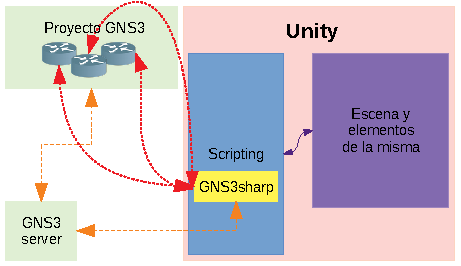
\includegraphics[scale=1.4]{imagenes/diagrama_interaccion}
  \caption{Diagrama de la interacción entre Unity y GNS3}
  \label{fig:diagrama_interaccion}
\end{figure}

Los colores de las flechas en la figura anterior son representativos. Mientras que las flechas naranjas establecen conexiones mediante REST (es decir, con conexiones HTTP), las rojas lo hacen con sockets. Así, la API solicita y envía información al servidor de GNS3 mediante sobre HTTP y hace lo propio con los nodos mediante sockets TCP.

Los proyectos de Unity están basados en un elemento llamado \GAOBJ. Todos los objetos que componen las escenas del proyecto se pueden abstraer en última instancia en ese tipo. El primer paso para que un proyecto de Unity pueda conectarse y controlar un esquema de red de GNS3 pasa por \textbf{insertar un \GAOBJ~ que tenga una instancia de la clase \GNSCS}. La única condición que se le impone a este objeto es que este parámetro contenido en él (la instancia) ha de ser accesible por todo el resto de elementos de la escena.

¿Para qué? De este modo, todos esos elementos no necesitan crear la suya propia. Creando una sola instancia de la clase centralizamos el trabajo en un solo objeto. La instancia contendrá información de los datos del proyecto de GNS3; información que podrá ser tomada por todos los componentes de la escena sin más que copiar la referencia al objeto. Si estos declararán su propia instancia cada uno perdería en tiempo (la recopilación de datos desde el servidor no es instantánea) y en eficiencia.

La idea es que el jugador (en otros términos, el usuario final), posea interacción con el simulador de redes de forma que \textbf{las consecuencias puedan verse reflejadas en el juego}. Pongamos un ejemplo e invirtamos el orden lógico de desarrollo para entender mejor cómo funcionaría esto:

\begin{enumerate}
\item El jugador se encuentra en una habitación que no es más que una \textbf{representación de un router}. Tiene un botón justo delante suya. En la pantalla se le avisa de que si lo pulsa, la puerta asociada a una determinada interfaz se cerrará, de forma que los enemigos que se ven acercarse en esa dirección no podrán pasar. Lo pulsa entonces.
\item Ese botón es un \GAOBJ~ de la escena actual que tiene un \textit{trigger} asociado a él y un script que lo gestiona. Uno de los atributos de tal código es la referencia a la instancia del objeto \GNSCS, construido al arrancar la escena y que suponemos ya contiene toda la información del proyecto de GNS3. Cuando se activa el trigger (una condición del script pasa a ser \texttt{True}), se toma la referencia del objeto asociado al router donde el personaje está. Se utiliza tal objeto para enviar un comando al router que le haga apagar la interfaz correspondiente.
\item El mensaje llega al router. Este lo ejecuta y devuelve el resultado.
\item El script recibe la respuesta y, tras analizarla, confirma que la interfaz se ha cerrado. Envía un mensaje al \GAOBJ~ de la puerta para que la cierre.
\end{enumerate}

Este flujo es lo que se ha representado en la figura~\ref{fig:diagrama_interaccion}. El bloque morado hace referencia a todo el entorno que comprende una escena de Unity. Esta escena contendrá una serie de \GAOBJ s, cuyo comportamiento vendrá determinado mayormente mediante lógica programada por scripts. El bloque azul hace referencia a este compendio. Alguno de esos scripts será el encargado de contener una instancia de \GNSCS . Al ser creada, esta se conecta al servidor de GNS3 desde donde recibe toda la información del proyecto con el que se quiere trabajar. A partir de ahí, el resto de \GAOBJ s de la escena no tendrán más que usar esa instancia para poder conectarse a los nodos (entre otras cosas) de la simulación. 

\subsection{Modelo de videojuego}\label{subsec:modelojuego}
Ahora que sabemos de qué forma se interconecta el juego con la red y en qué consiste exactamente la interacción, queda por concretizar qué clase de juegos podríamos crear. Hay que tener en mente en todo momento que pretendemos crear un \textbf{juego didáctico}, así que no nos vale cualquier construcción. La dificultad es, entonces, doble, pues es necesario seguir los cánones que dictan el buen hacer de un videojuego (véase un inteligente diseño de niveles, una estética atractiva y coherente, apartado técnico gráfico y sonoro propio, niveles a prueba de bugs...) a la vez que planear \textbf{qué} se quiere enseñar en ellos y \textbf{cómo} se pretende hacerlo.

Para sortear estas dificultades se ha decidido que la estructura del juego esté basada en pequeños niveles interconectados entre sí por una plataforma común. La linealidad de un juego exige de un guion y de una cohesividad de los que el juego ``federado'' puede permitirse  prescindir.

\begin{figure}[H]
  \centering
  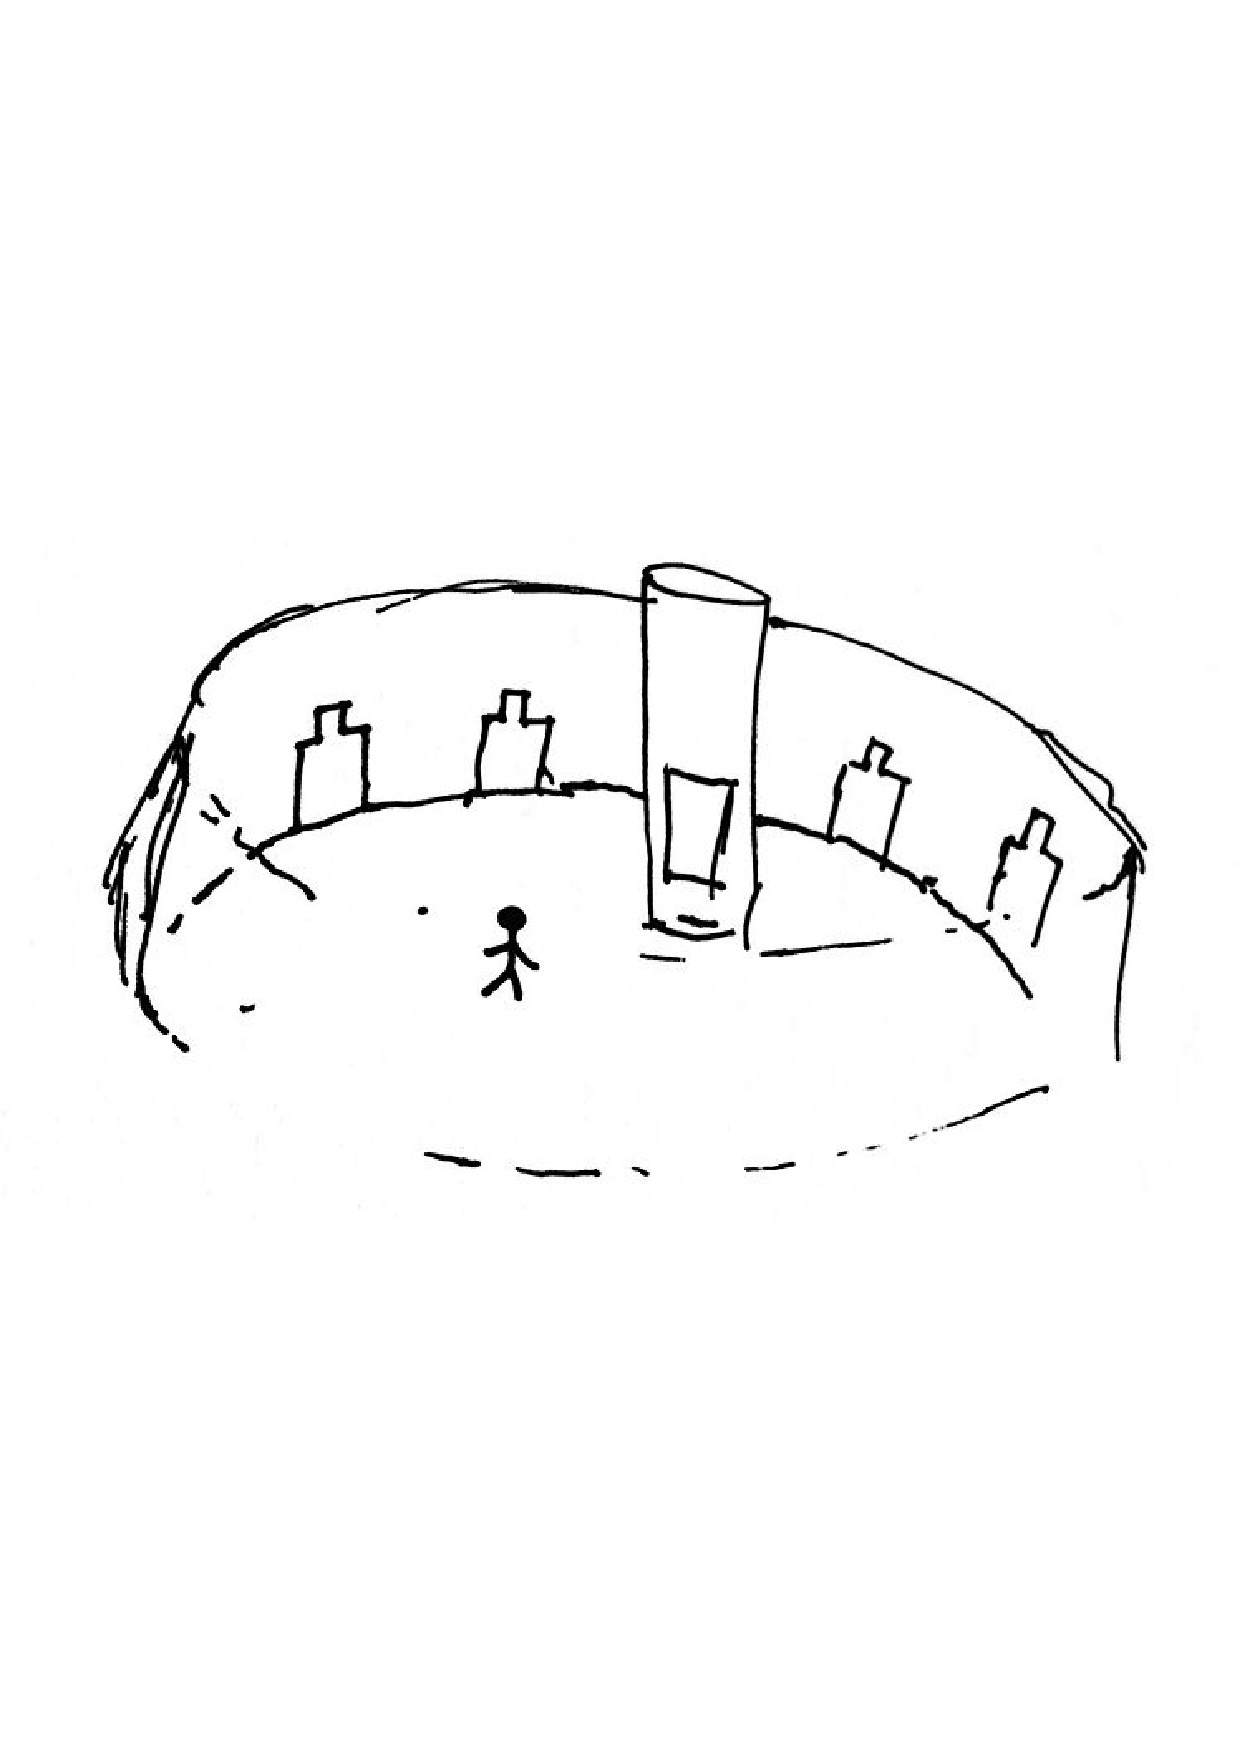
\includegraphics[scale=0.35, trim={0 9cm 0 9cm}]{imagenes/hall_juego}
  \caption{Boceto de la sala de distribución del juego}
  \label{fig:hall}
\end{figure}

En el boceto de la figura de arriba se quiere ejemplificar (de forma extremadamente simplista) en qué consistiría este diseño.
\begin{itemize}
\item Cada vez que el jugador entre en el juego se encontrará en una suerte de sala de distribución. Esta estará acotada por paredes con un número determinado de puertas.
\item Estas puertas conducen a los distintos niveles del juego. Cada puerta corresponde a una lección diferente sobre redes y telemática. El jugador no tiene que superar una lección (un nivel, una zona) para acceder a la siguiente, sino que puede elegir qué quiere aprender indistintamente. Por supuesto, se podría vetar la entrada a una zona hasta que supere una concreta. Idealmente, cada nivel al que se accede contaría con varias fases que van incrementando en dificultad.
\item Al superar estas zonas, se desbloquea un ``manual'' acerca de lo aprendido en esa sala. Este manual puede ser consultado en un monitor localizado en el centro del hall. Gracias a esto, se podría repasar rápidamente lo aprendido en niveles anteriores desde un solo lugar.
\end{itemize}
Esta forma de acceder a los niveles es similar a la que siguen los videojuegos de la saga \textit{Crash Bandicoot} (\textit{2}, \textit{3}, \textit{La venganza de Cortex...}), donde existe una sala de ``descanso'' desde la que elegir cuál será la siguiente fase a jugar. Abstrayendo esta idea algo más, no es más que un menú estático desde donde elegir el nivel (juegos de corte más ``clásico'' como \textit{Super Meat Boy} utilizan este patrón) salvo que gozando de una interacción más directa y natural con el jugador, integrándolo más.

Existen dos aproximaciones al modo en el que estos niveles se conectan con el simulador de redes:
\begin{itemize}
\item Por un lado, podría existir \textbf{un proyecto de GNS3 por cada nivel} y/o fase. Aunque mucho más estructurado y por ende posiblemente más sencillo de gestionar, es necesario establecer conexión con el servidor de GNS3 por cada nivel para recopilar la información del mismo. Esto se traduce en tiempo. Además, el servidor de GNS3 no registra el proyecto de GNS3 a menos que este se abra manualmente desde GNS3 en una sesión. Más tiempo.
\item La otra solución pasa por crear \textbf{un solo proyecto} para todo el juego. Sería necesario desplegar todos los aparatos que vayan a ser utilizados en él, incrementando altamente los recursos que el sistema utiliza. Para paliar este último problema existen dos opciones:
\begin{enumerate}
\item Encender los aparatos que vayan a ser necesitados en el nivel a jugar y cerciorarse de que el resto permanece apagado.
\item Reconfigurar los aparatos que vayan a ser utilizados para que sus propiedades se correspondan a lo que se necesita para el respectivo nivel.
\end{enumerate}
De entre estos dos acercamientos al problema, quizás el primero sea más simple, pero el arranque de cada nodo no es inmmediato. El segundo entraña una mayor dificultad ingenieril y mayor propensión al error aunque la configuración de los aparatos conlleve menos tiempo.
\end{itemize}

\subsection{Caso de ejemplo}\label{subsec:fracasojuego}

Sin embargo, aunque todas estas ideas pueden sonar realmente interesantes, el juego final desarrollado no ha podido alcanzarlas. La complejidad existente para llevarlo a cabo era demasiado grande. En su lugar, se ha preferido crear un único pequeño escenario que sirva como demostración del potencial del proyecto.

Con este propósito, se desarrollará un minijuego basado en tablas de enrutamiento. El objetivo del jugador es ser capaz de alcanzar un dispositivo marcado de la red en el menor tiempo posible. Por supuesto, habrá de atravesar una serie de nodos para alcanzarlo.

El mapa estará compuesto por varias plataformas y en cada una de ellas un cartel con la tabla de enrutamiento del respectivo router. Son estas plataformas entonces una suerte de representantes de los routers de la red. Al jugador se le darán varias posibles opciones como siguiente salto. Cada opción es una interfaz del router. En la interfaz aparecerá la dirección IP del equipo a alcanzar. El resultado será similar a lo que puede verse en la figura \ref{fig:juegoaccion}.

\begin{figure}[H]
  \centering
  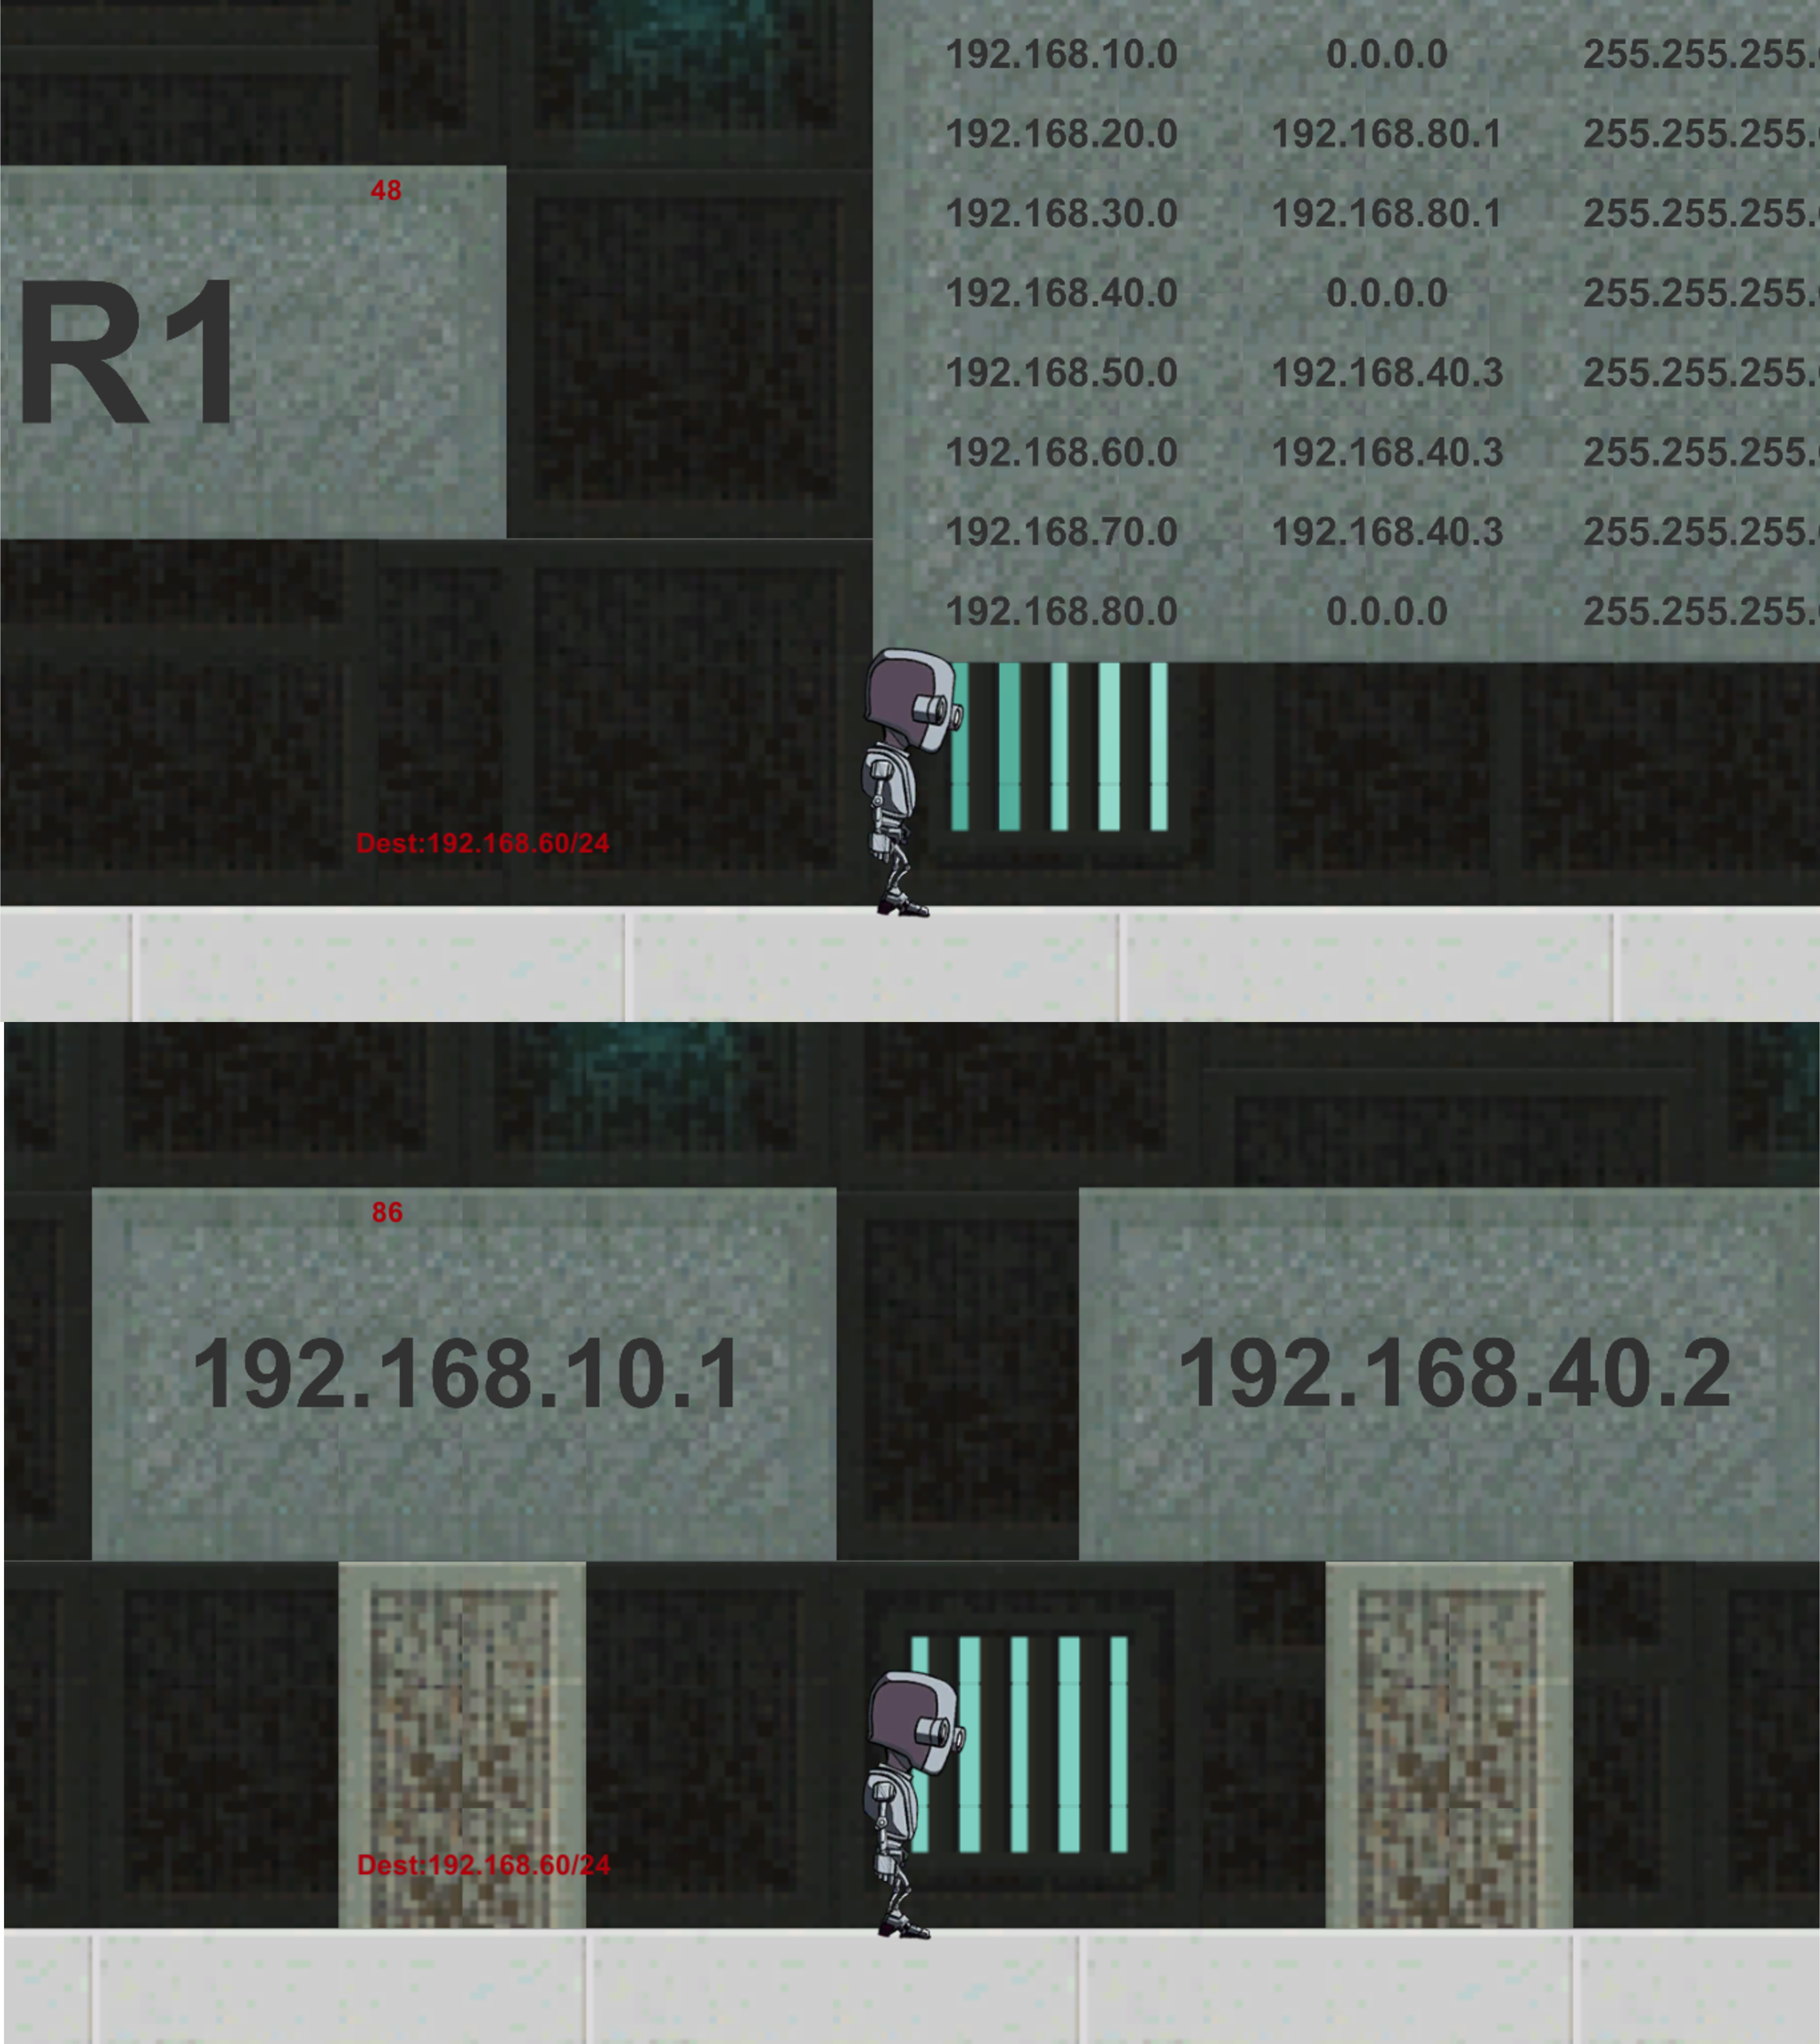
\includegraphics[scale=0.1]{imagenes/juegoaccion}
  \caption{Imágenes del minijuego en acción}
  \label{fig:juegoaccion}
\end{figure}

Con este nivel tan sencillo conseguimos dos cosas:
\begin{itemize}
\item Dar un ejemplo de juego didáctico con redes. Se ponen a prueba los conocimientos del jugador sobre redes y se le anima a hacerlo lo mejor posible a través de un contador ascendente.
\item Mostrar cómo se lleva a cabo la interacción entre el simulador y el juego. Dicho en otras palabras, demostrar que, efectivamente, la API es funcional y puede ser usada con el propósito que se esperaba.
\end{itemize}

Se cimentan unos pilares sobre los que podrán construirse cosas mucho mayores en el futuro.